\chapter{The acquisition of data}

\section{The LHC}
LHC is a big boy detector in geneva. Magnets move particles about, very cool.  
\subsection{What gets made?}
\begin{figure}[h!]
  \centering
  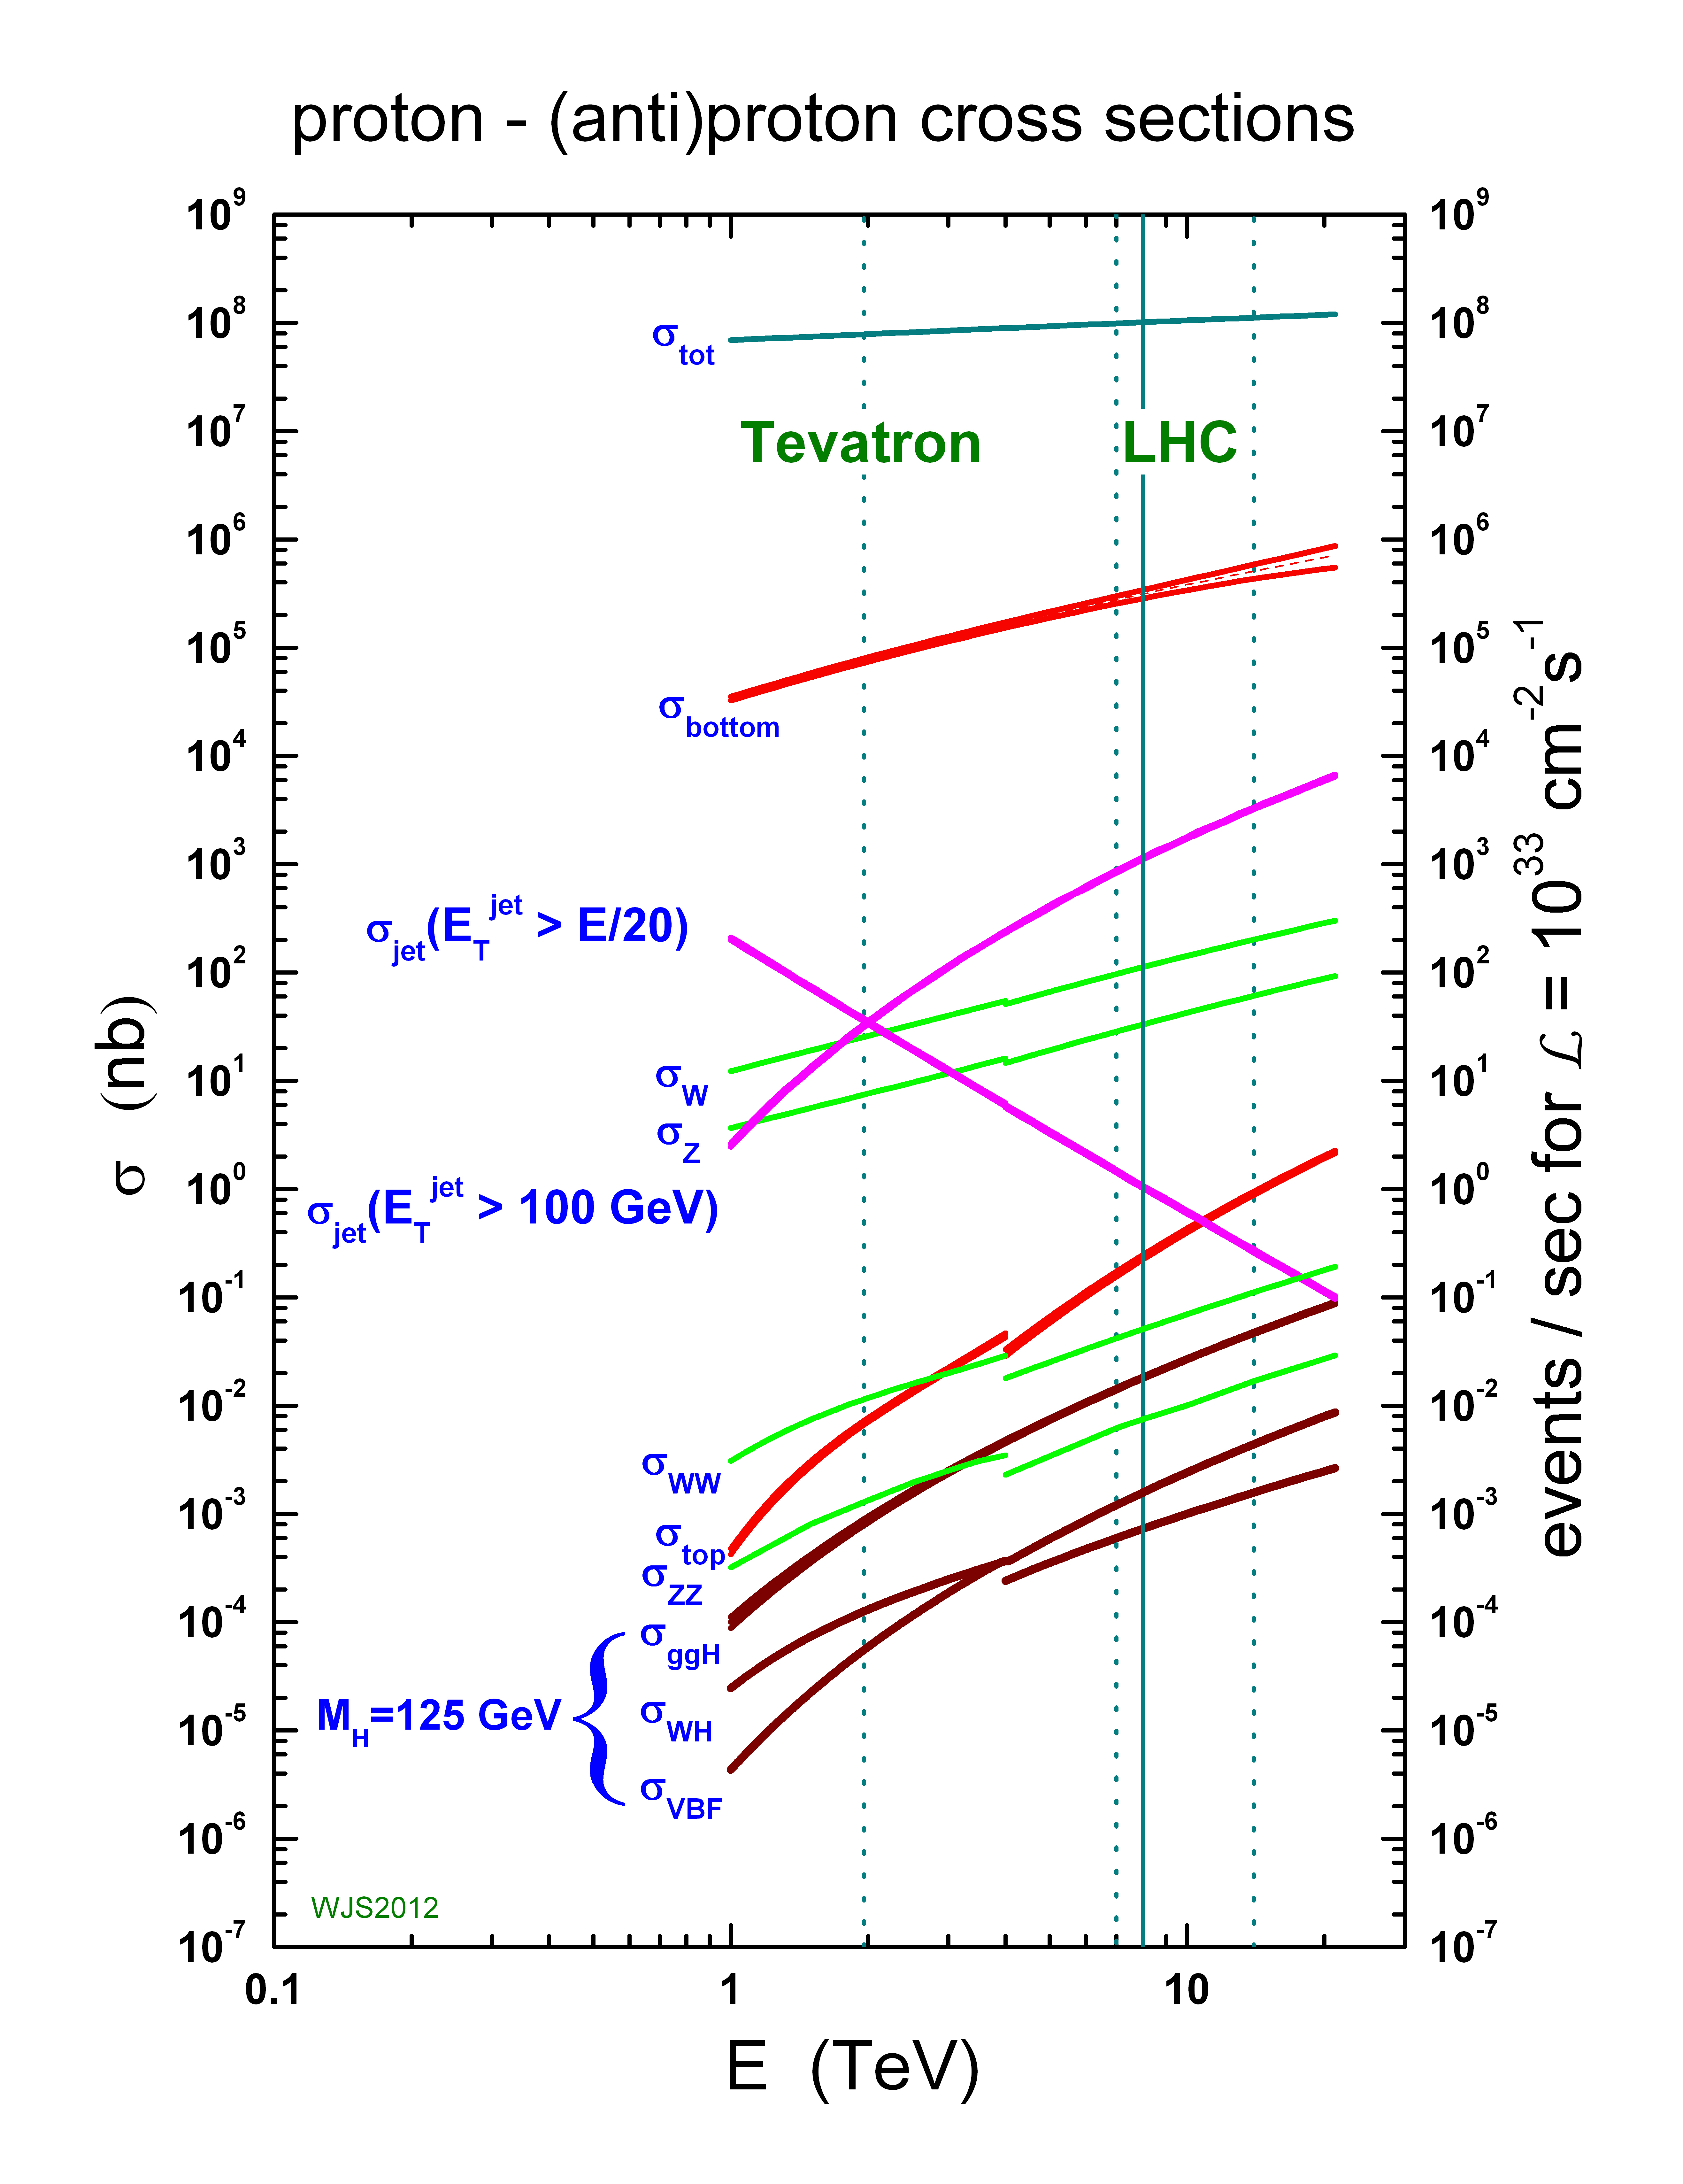
\includegraphics[width=.7\textwidth]{figures/lhc_decay_modes.jpg}
  \caption{Production Cross Sections for the LHC}
  \label{fig:lhc_decay_modes}
\end{figure}

Point out that there is very low chance for double scattering or two interesting interactions in one bunch crossing. Point out cross section of Z boson, point out the NJets rule.

\section{The CMS Detector}
\subsection{The Inner Tracker}
\subsection{The Electromagnetic Calorimeter}
\subsection{The Hadronic Calorimeter}
\subsection{The Muon System}
\subsection{Fiducial Area}
the wierd eta deadzone, very forward stuff.
\subsection{Event Triggering} \label{sec:event_triggering}
trigger turn ons, list the triggers we use, Level 1 and HLTs?


\section{Physics Objects}
\subsection{Particle flow and event clustering} \label{sec:particle_flow}
\subsection{Vertex Selection}
\subsection{B-Tagging}
\subsection{Electron Measurement Pipeline} \label{sec:electron_measurement_pipeline}
Tracker, ecal, distinguishing between electrons and muons. Cite the CMS paper on electron energy reco..
\subsection{Muon Measurement Pipeline} \label{sec:muon_measurement_pipeline}
Tracker muons, global muons, muon system
\subsection{Photon Measurement Pipeline}
ECAL measurements, lepton conversions.
\subsection{Lepton Selection and Isolation}
Give iso and ID requirements, try to give justification for each
\subsection{Isolated Tracks}
Explain the selection and the rationale. The extra lepton veto could be good to mention here too. 
\subsection{MET Reconstruction} \label{sec:MET_reco}
  Make sure to add bits about sources of MET and the Type 1 correction
\subsection{Event Discriminators}
  We apply certain filters that kill events, these are called MET filters but include things like beam halo as well.

\section{Monte Carlo}

\section{Datasets} \label{sec:datasets}
We use dilepton trigger events, as will be described in section \ref{sec:leptonic_final_states}